\documentclass[10pt]{article}
\usepackage[utf8]{inputenc}
\usepackage{parskip}
\usepackage[margin = 1in]{geometry}
\usepackage{xcolor}
\usepackage[colorlinks = true,linkcolor = blue, urlcolor  = blue,citecolor = blue,anchorcolor = blue]{hyperref}
\usepackage{framed}
\usepackage{apacite}
\usepackage[authoryear,sort]{natbib}
\usepackage{amsmath}
\usepackage{amssymb}
\bibliographystyle{apalike}
\newcommand{\E}{\textrm{E}}
\newcommand\bref[2]{\href{#1}{\color{blue}{#2}}}
%\renewcommand*{\theenumi}{\thesection.\arabic{enumi}}
\renewcommand{\P}{\text{P}}
\usepackage{tikz}
\usetikzlibrary{arrows,shapes.arrows,positioning,shapes,patterns,calc}

\begin{document}

\begin{Large} 
Info 6751. Fall 2022. Problem Set 12. Due on Canvas by 5pm on 22 Nov (Note: Tuesday deadline. Final proposal due Monday!).
\end{Large}
\hline \vskip .1in

Note: This assignment is brief so you can work on your research proposal.

This problem set works with the causal structure in the following DAG. Further, we assume this is a linear structural equation model: the causal effect represented by each edge corresponds to a coefficient which is the same for every unit. In every case, assume estimation is with OLS.

\begin{center}
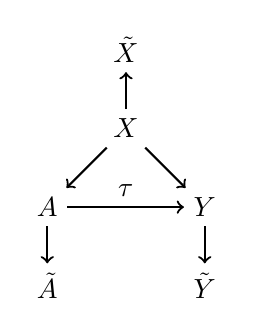
\begin{tikzpicture}
\node (a) at (0,0) {$A$};
\node (y) at (2,0) {$Y$};
\node (atilde) at (0,-1) {$\tilde{A}$};
\node (ytilde) at (2,-1) {$\tilde{Y}$};
\node (x) at (1,1) {$X$};
\node (xtilde) at (1,2) {$\tilde{X}$};
\draw[->, thick] (a) -- node[midway, above] {$\tau$} (y);
\draw[->, thick] (x) -- (a);
\draw[->, thick] (a) -- (atilde);
\draw[->, thick] (y) -- (ytilde);
\draw[->, thick] (x) -- (y);
\draw[->, thick] (x) -- (xtilde);
\end{tikzpicture}
\end{center}

\begin{enumerate}
\item (10 points) A researcher measures $\{\tilde{X},A,Y\}$. They estimate the causal effect of $A$ on $Y$ by regressing $Y$ on $\{\tilde{X},A\}$. Is their estimator consistent for $\tau$?
\item (10 points) In (1), what backdoor path remains unblocked?
\item (10 points) In (1), suppose $X\rightarrow A$ and $X\rightarrow Y$ are positive causal effects. What can you say about the direction of the bias arising from the backdoor path that is imperfectly blocked?
\item (10 points) Suppose all variables are standardized and the standardized coefficient on $X\rightarrow A$ equals the standardized coefficient on $X\rightarrow \tilde{X}$. In this setting, would you prefer the control estimator or the difference estimator in \bref{https://doi.org/10.1177/0049124119875958}{Elwert \& Pfeffer (2022)}? If you are stuck, see Fig 2 and 3 in that paper.
\item (10 points) Tell a story for this structure. Define substantive variables that could be $\{X,A,Y\}$ and give reasons why they might be measured with error as in the figure.
\end{enumerate}

\end{document}

